\begin{document}

\maketitle

\section{Sissejuhatus}
\begin{frame}[fragile]
  \frametitle{Eelmine kord}
  Keerulised teemad, rõhk keeruliste süsteemide käitumisel eri olukordades
	\begin{itemize}
		\item Jätkusuutlikkus on oluline teema, kui pealispinna alla vaadata
		\item Muudatused äris on vältimatud, nende tagajärjed ITle mittetriviaalsed
		\item Riskijuhtimine klassikalisel kujul keeruliste süsteemide puhul ei toimi
	\end{itemize}
\end{frame}

\begin{frame}[fragile]
  \frametitle{Täna kavas}
		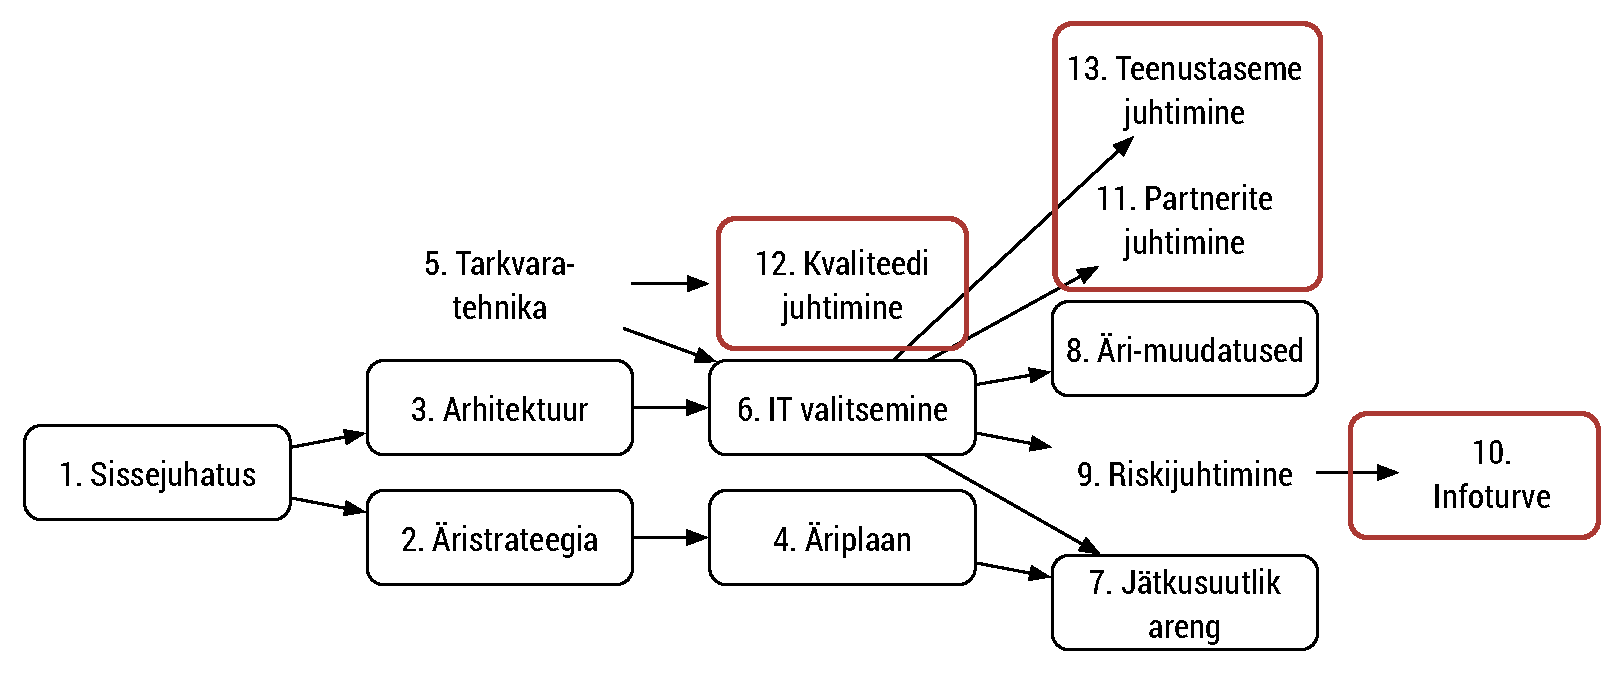
\includegraphics[width=\textwidth]{aine_struktuur_neljas.pdf}
\end{frame}

\section{Infoturve}
\begin{frame}[fragile]
  \frametitle{Küberründe võrratus}
	\begin{center}
	  Rünne tasub end ära siis ja ainult siis, kui:\par
		$S_p>P_f(S_a + P_c S_c)$
	\vfill
	\begin{description}
		\item[$S_p$] Ründest oodatav kasu
		\item[$P_f$] Ründe ebaõnnestumise tõenäosus
		\note{Ründe ebaõnnestumise tõenäosus on reaalselt alati väiksem kui üks: küsimus ei ole sisse saamises, küsimus on kiiruses, hinnas ja sügavuses. Kui otse rünnatakse, siis ka maha võetakse}
		\item[$S_a$] Ründe läbi viimise kulu
		\item[$P_c$] Vahele jäämise tõenäosus
		\item[$S_c$] Vahele jäämise kulu
	\end{description}
	\end{center}

\end{frame}

\begin{frame}[fragile]
  \frametitle{Muutujate seis}
	\begin{itemize}
		\item $S_p$ kasvab, kuna 
			\begin{itemize}
				\item Andmeid saab kasutada (ka) järgmise rünnakute jaoks (tagasiside) 
				\item Interneti sõltuvus reklaamist ja seega privaatsest infost kasvab
				\item Eksisteerib toimiv andmete ja ründeteenuste must turg
			\end{itemize}
		\item $P_f$ kahaneb, kuna süsteemid lähevad järjest keerulisemaks
		\item $S_a$ on dramaatiliselt langenud, kuna 
			\begin{itemize}
				\item Ründed on paljus automatiseeritud
				\item Eksisteerib toimiv üle võetud arvutite must turg
				\item Toimib tagasiside: mida rohkem arvuteid üle võetakse, seda rohkem arvuteid suudetakse rünnata ja seega ka üle võtta
			\end{itemize}
		\item $P_c$ arenenud riikides kasvab, mujal stabiilne
		\item $S_c$ arenenud riikides kasvab kiiresti (vt. megauploadi juhtum)
	\end{itemize}
	\note{Võrratuse parem pool kasvab, kuna ründed lähevad odavamaks ja efektiivsemaks palju kiiremini, kui kasvab vahele jäämise tõenäosus}
\end{frame}


\begin{frame}[fragile]
  \frametitle{Võrratuse tulemus}
	Üksikud intsidendid on asendunud pideva vooga
	\begin{itemize}
		\item Põhjuseks rünnete hinna langemini kiiremini, kui suudetakse tõsta vahele jäämise kulusid
		\item CERT-EE hinnagul ei ole 2015 aasta alguseks enam märgata pause \emph{(spear) phishingu} kampaaniate vahel
		\item Väga suurt rolli mängib automatiseerimine: kuigi automatiseeritud või \emph{drive-by} ründe $P_f$ on suhteliselt suur, on $S_a$ sisuliselt null
	\end{itemize}
\end{frame}

\begin{frame}[fragile]
  \frametitle{Turvalisus ja arhitektuur}
	\begin{center}
		Ohutus (rurvalisus) ei ole mitte süsteemi funktsioon vaid selle emergentne käitumine
		\note{Turvalisust ei saa funktsionaalsete nõuete kaudu väljendada. Saab nõuda teatud testide läbi viimist ja saab püstitada ohutusnõuded, kuid ohutust kui sellist ei saa ei nõuda ega testida.}
	\end{center}
	\cite{leveson2011engineering}
\end{frame}

\begin{frame}[fragile]
  \frametitle{Turvalisus tuleb arhitektuurist}
	Turvalisus peab olema sisse ehitatud süsteemi arhitektuuri
	\begin{itemize}
		\item Seda ei saa hiljem lisada ega "külge kruvida"
		\item Kuna me ei suuda emergentsust kontrollida, on turvalisuse tagamine süsteemi elutsüklit läbiv protsess: Ohuanalüüsi tulemid on sisendiks disainiotsustele mis realiseerituna omakorda annavad sisendi uuele ohuanalüüsile
		\item Olulisel kohal on süsteemi kontseptsioon: kas idee on toetuda ühe sõlme turvalisusele või on terve süsteem ehitatud vastupidavaks?
		\note{Lõuna-Korea isikukoodi näide\par}
	\end{itemize}
\end{frame}

\begin{frame}[fragile]
  \frametitle{Infoturbe strateegiast}
	Mõned infoturbe strateegilised aspektid:
	\begin{itemize}
		\item Oluline on määratleda (ja kommunikeerida) aktsepteeritud riskitase
		\begin{itemize}
			\item Kuigi nuga on ohtlik, on ta meil siiski enamasti olemas
			\note{Kasulikkus kompenseerib riski\par}
			\item Järelikult peab olema paigas (kommunikatsiooni) plaan riski realiseerumise puhuks
		\end{itemize}
		\item Strateegiline roll on kogukonnal:
		\begin{itemize}
			\item Süsteemi olulised komponendid ei ole tingimata teie kontrolli all
			\item Tundliku info jagamise aluseks on usaldus
			\note{õige käitumise aluseks on õigeaegne info\par}
			\item Internet on liiga terviklik süsteem, et võiks üksi asju ajada
			\note{Seepärast CERTide võrk tekkiski\par}
			\item Panustage ja te saate vastu
			\note{küberkaitseliit ja muud kogukondlikud ettevõtmised. Selle eelduseks on, et teil on inimesed, kes on suutelised reaalselt panustama\par}
		\end{itemize}

	\end{itemize}
\end{frame}


%Arutelu koht
\begin{frame}[fragile]
  \frametitle{Arutelu koht}
		\begin{center}
			\textbf{Kuidas tellida turvalist tarkvara?}
		\end{center}
\end{frame}

\section{Partnerite juhtimine}
\begin{frame}[fragile]
  \frametitle{Partnerite juhtimine}
	\begin{itemize}
		\item Hinda realistlikult oma võimet partnerit juhtida. Jaapani näide. 
		\item Kui vähegi kahtlus, ära juhi partnerit. Sun Tzu tsitaat. Strateegiad:
			\begin{itemize}
				\item Ignoreeri kogu probleemi (kohvi ja vetsupaber)
				\item Juhi tehnoloogiat
				\item Juhi/kasuta standardeid
				\item Juhi kogukonda
				\item Jaga ja valitse
			\end{itemize}
	\end{itemize}
\end{frame}

%Arutelu koht
\begin{frame}[fragile]
  \frametitle{Arutelu koht}
		\begin{center}
			\textbf{2. küsimus}
		\end{center}
\end{frame}

\begin{frame}[fragile]
  \frametitle{Partnerite juhtimine}
  Kui muud moodi ei saa
	\begin{itemize}
		\item Räägi riskijuhtidega. Partneril on strateegiline roll riskides
		\item Ökosüsteemi, mitte üksiku partneri vaade. Kes veel on mängijad, mis on nende huvid?
		\item Partneri juhtimise aluseks on võime ennast juhtida. Nagu ka inimeste puhul. Rõhuv enamus "partner on loll" olukordi minu kogemuses tulenevad otseselt kliendi võimekusest kliendina käituda. Kord kaotatud strateegilist positsiooni on väga raske tagasi võita (teadmuskao tagasiside)
		\item Kliendina käitumiseks kriitiline
			\begin{itemize}
				\item Kontroll IP üle. Nii tehniline kui sisuline!
				\item Kontroll arhitektuuri üle
				\item Kontroll lepingu ja selle täitmise üle. Iga ebatäpsust siin kasutatakse ära
			\end{itemize}		
		\item Kehtestav käitumine: oma vajaduste selge ja järjekindel väljendamine ning nende eest seismin
	\end{itemize}
\end{frame}

%Arutelu koht
\begin{frame}[fragile]
  \frametitle{Arutelu koht}
		\begin{center}
			\textbf{3. küsimus}
		\end{center}
\end{frame}

\section{Kvaliteedi juhtimine}

\begin{frame}[fragile]
  \frametitle{Kvaliteedi juhtimine}
	Miks tarkvaras on vead
	\begin{itemize}
		\item Vigade parandamise dünaamiline mudel, selle matemaatiline lahend
		\item Mudeli järelmid: alati on veel vigu, testima tuleb hakata vara
		\item Otsustuskriteeriumid lõpetamiseks: eraldame ratsionaalse ja irratsionaalse. Ratsionnalselt (graafik): kui oleme jõudnud allapoole spetsifikatsiooni veamarginaali
	\end{itemize}
\end{frame}

%Arutelu koht
\begin{frame}[fragile]
  \frametitle{Arutelu koht}
		\begin{center}
			\textbf{4. küsimus}
		\end{center}
\end{frame}

\begin{frame}[fragile]
  \frametitle{Kvaliteedi juhtimine}
	Jaapanlaste lähenemine
	\begin{itemize}
		\item Seos lean liikumisega
		\item Kaizeni olemus
		\item Teede parandamise näide
		\item Selle järeldused tarkvaratehnika ja QA jaoks
	\end{itemize}
\end{frame}

%Arutelu koht
\begin{frame}[fragile]
  \frametitle{Arutelu koht}
		\begin{center}
			\textbf{5. küsimus}
		\end{center}
\end{frame}


\section{Teenustaseme juhtimine}
\begin{frame}[fragile]
  \frametitle{Teenustaseme juhtimine}
	\begin{itemize}
		\item Teenustaseme juhtimise aluseks on teenuse mõiste olemasolu (alignment kõigis kihtides)
		\item Arutelu teenustasemete üle riskijuhtimist kaasamata on lihtsalt grupp jonnivaid inimesi
		\item Teenustase tuleb määratleda läbi riskide
		\item Järelikult tuleb mõõta teenust, mitte masinaid. Masinad, nagu rääkisime, lähevad ennustataval viisil katki
		\item Keerulist süsteemi modelleerima hakka ainult siis, kui sul on palju aega ja raha ning tõsine vajadus. Sest ta on keeruline. Ja, nagu rääkisime, teenustaseme kao põhjus võib olla mõõtmisvea lähedal ja seega raskesti mürast eristatav
	\end{itemize}
\end{frame}


%Arutelu koht
\begin{frame}[fragile]
  \frametitle{Arutelu koht}
		\begin{center}
			\textbf{6. küsimus}
		\end{center}
\end{frame}


\section{Viited}

\begin{frame}[t,allowframebreaks,]
  	\bibliographystyle{plainnat}
	\bibliography{it_strateegia} 

\end{frame}

%\plain{Küsimusi?}
\begin{frame}[plain]
	\begin{center}Küsimusi?\end{center}
\end{frame}


\end{document}